\documentclass[12pt,a4paper]{article}
\usepackage[utf8]{inputenc}
\usepackage[T1]{fontenc}
\usepackage[english]{babel}
\usepackage{graphicx}
\usepackage{geometry}
\geometry{a4paper,left=25mm,right=25mm,top=25mm,bottom=25mm}
\usepackage{amsmath} % Matematik formülleri için
\usepackage{enumitem} % Madde listeleme için
\usepackage{hyperref} % İçindekiler kısmı için tıklanabilir bağlantılar
\usepackage{sectsty} % Control sectional headers.
\usepackage{float} % For [H] float placement
\sectionfont{\centering} % center section headers

% Özel komutları tanımlayın
\newcommand{\projecttitle}{GrammarGraph: Dynamic AST Generator} % Proje başlığı
\newcommand{\studentname}{Elanur Kurt, Eylül Kalfa, İrem Su Köse} 
\newcommand{\studentnumber}{439199, 439184, 439183} % Öğrenci numaraları

\title{\projecttitle}
\author{\studentname \\ \studentnumber}
\date{\today}

\begin{document}
	
	
	\begin{titlepage}
		\centering
		
\includegraphics[width=0.50\textwidth]{KTU_Logo_2A.png} 
		\vspace{1cm}
		
		\textbf{\large KARADENIZ TECHNICAL UNIVERSITY}\\ \vspace{1mm}
		\textbf{\large FACULTY OF ENGINEERING}\\ \vspace{1mm}
		\textbf{\large  DEPARTMENT OF SOFTWARE ENGINEERING}\\

		\vspace{1cm}
		
		{\large \textbf{\MakeUppercase{\projecttitle}}} \\
		\vspace{1.5cm}
		
		{\large \textbf{Student Names:} \studentname} \\
		{\large \textbf{Student Numbers:} \studentnumber} \\
		\vspace{1cm}
		
		{\large \textbf{Date:} \today} \\
		\vfill
	\end{titlepage}
	

	\tableofcontents
	\newpage
	

	\section*{Abstract}
	This project presents the implementation of a custom Syntax Analyzer and Parse Tree Visualizer developed in Python for analyzing Context-Free Grammars (CFGs) written in Backus-Naur Form (BNF). The system reads grammar rules from external text files, tokenizes input sentences, validates whether the token sequences conform to the given grammar, and generates corresponding parse trees. The parser is implemented using the Recursive Descent Parsing technique, which follows a top-down parsing strategy. 

The project supports both standard English sentence structures and grammars containing epsilon ($\varepsilon$) productions. Additionally, the system provides detailed error reporting mechanisms for invalid sentences, including token position, expected grammar rules, and descriptive rejection messages. Valid parse results are represented in multiple formats, including hierarchical console output, nested JSON structures, and graphical Abstract Syntax Tree (AST) visualizations generated with Graphviz and pydot libraries.

The implementation demonstrates practical applications of formal language theory, recursive parsing algorithms, compiler design concepts, and data structure usage in syntax analysis systems.
	\subsection*{Keywords}
	Context-Free Grammar, Recursive Descent Parser, Syntax Analyzer, Parse Tree, Abstract Syntax Tree, BNF, Python, Compiler Design, Graphviz, JSON
	
	
	\section{Introduction}
	Programming languages rely heavily on syntax analysis to determine whether a sequence of tokens conforms to a predefined grammar. Syntax analyzers, also known as parsers, are essential components of compilers, interpreters, and language-processing systems. They validate input structures and generate internal representations such as parse trees or abstract syntax trees.

The purpose of this project is to develop a custom Syntax Analyzer and Parse Tree Visualizer using Python. The system is designed to read Context-Free Grammar (CFG) rules written in Backus-Naur Form (BNF) from external text files and analyze whether given sentences conform to these rules.

If the input sentence is syntactically valid, the parser generates:
\begin{itemize}
    \item A hierarchical text-based parse tree,
    \item A nested JSON representation,
    \item A graphical Abstract Syntax Tree (AST) visualization in PNG format.
\end{itemize}

If the sentence is invalid, the system provides detailed and user-friendly error messages instead of terminating unexpectedly.

The project focuses on several important concepts in programming language theory and compiler construction:
\begin{itemize}
    \item Context-Free Grammars (CFG),
    \item Recursive Descent Parsing,
    \item Abstract Syntax Trees,
    \item Recursive algorithms,
    \item Error handling mechanisms,
    \item Data structure design.
\end{itemize}

The implementation was developed entirely in Python and uses external libraries such as Graphviz and pydot for visualization purposes.

\section{Project Objectives}

The main objectives of this project are:

\begin{enumerate}
    \item To design a syntax analyzer capable of reading BNF grammar rules dynamically from text files.
    
    \item To implement a Recursive Descent Parser using top-down parsing techniques.
    
    \item To validate whether token sequences conform to the specified grammar.
    
    \item To support grammars containing epsilon ($\varepsilon$) productions.
    
    \item To generate parse trees both textually and graphically.
    
    \item To produce machine-readable JSON representations of parse trees.
    
    \item To implement detailed error handling mechanisms for invalid inputs.
    
    \item To demonstrate the practical use of formal language theory and compiler construction concepts.
\end{enumerate}
	\section{Aims and Objectives}
	The primary aim of this project is to develop a custom Syntax Analyzer and Parse Tree Visualizer using Python for processing Context-Free Grammars (CFGs) written in Backus-Naur Form (BNF). 

The objectives of the project are:
\begin{itemize}
    \item To read grammar rules dynamically from external text files,
    \item To implement a Recursive Descent Parser for syntax analysis,
    \item To validate whether input sentences conform to the given grammar,
    \item To generate parse trees in textual, JSON, and graphical formats,
    \item To support grammars containing epsilon ($\varepsilon$) productions,
    \item To provide detailed and user-friendly error handling for invalid inputs.
\end{itemize}
	
	\section{Methodology}
	This section describes the methods and procedures used in our project. For the SE2002 Programming Languages course, we developed a Recursive Descent Parser in Python to meet the "Expression Evaluation and Selector Design" requirements. During the development process, we did not follow a strict division of labor or a sequential model. Instead, our team consisting of Elanur Kurt, İrem Su Köse, and Eylül Kalfa came together at all stages to brainstorm, and we completed the algorithm design and coding processes by working collaboratively.

The system consists of a modular structure that can dynamically read grammar rules from an external file, check whether the given sentences or word sequences comply with these rules, and generate an Abstract Syntax Tree (AST) if they are appropriate.

\subsection{Grammar Rules Representation}
Our parser processes structured grammar rules as terminal and non-terminal expressions. Table \ref{tab:terminals} shows some of the basic word types and terminal options recognized by the system.

\begin{table}[h!]
    \centering
    \begin{tabular}{|l|l|}
       
        \hline
        \textbf{Non-Terminal Expression} & \textbf{Terminal Options} \\
        \hline
        \textless determiner\textgreater & the, a \\
        \hline
        \textless pronoun\textgreater & he, she, it, they, me, you \\
        \hline
        \textless adjective\textgreater & big, small, happy, lazy, red \\
        \hline
        \textless verb\textgreater & saw, liked, admired \\
        \hline
         
         \textless conjunction\textgreater & and, or \\
          \hline
         \textless adverb\textgreater & quickly,slowly,carefully,loudly \\
          \hline
         \textless noun\textgreater & cat,dog,man,telescope \\
         \hline
    \end{tabular}
    \caption{Sample Grammar Terminals}
    \label{tab:terminals}
\end{table}

\subsection{Abstract Syntax Tree Output}
Below is an example of the tree output generated by the system:

\begin{figure}[h!]
    \centering
   
    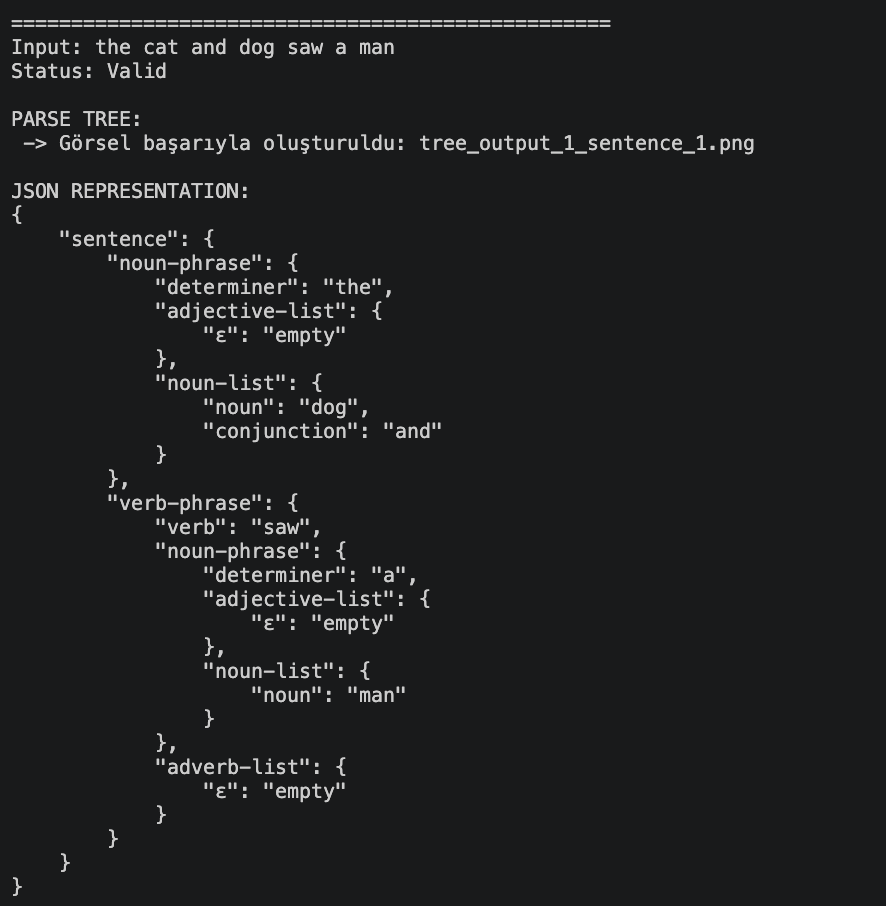
\includegraphics[width=1.0\textwidth]{ast_output.png} 
    \caption{Sample Abstract Syntax Tree (AST) output generated for the sentence "the cat and dog saw a man"  using the print\_tree function in nodes.py.}
    \label{fig:ast_example}
\end{figure}

\subsection{Recursive Grammar Parsing}
Our system can successfully parse recursive rules read from grammar files. For example, the production function of rule A  can be mathematically expressed as:
\[
A \rightarrow aA \mid \epsilon
\]
Here, $a$ represents a terminal, and $A$ represents a non-terminal that can recursively call itself. The empty string condition is denoted by $\epsilon$.

\subsection{System Modules}
Our project is shaped around three main modules in accordance with Object-Oriented Programming (OOP) principles:

\begin{itemize}
    \item \textbf{grammar\_reader.py}: Reads the rules from .txt files line by line, parses the left (lhs) and right (rhs) sides using the $::=$ and $|$ operators, and converts the system into a dictionary structure.
    \item \textbf{nodes.py}: Contains the Node class representing each element of the tree created during the parsing process. It manages child nodes and provides a hierarchical tree drawing (print\_tree) on the terminal screen.
    \item \textbf{parser\_logic.py}: The main parser that manages the system. It validates sentences according to grammar rules. It also includes a custom error-handling mechanism that deeply reports the missing structure ("expected") and the reason for the error ("reason") when an unexpected situation is encountered.
\end{itemize}
	\section{Findings}
	The developed syntax analyzer successfully parsed and validated multiple input sentences based on the provided Context-Free Grammar (CFG) rules. The system was tested using both standard English sentence grammars and recursive grammars containing epsilon ($\varepsilon$) productions.

The parser correctly identified valid and invalid inputs while generating detailed parse tree structures. For valid sentences, the program produced:
\begin{itemize}
    \item Hierarchical text-based parse trees,
    \item Nested JSON representations,
    \item Graphical parse tree visualizations in PNG format.
\end{itemize}

Additionally, the error handling mechanism successfully detected syntax mismatches and provided descriptive error messages indicating the exact error position and expected grammar rule.

\subsection{Sample Parsing Results}

\begin{table}[H]
\centering
\begin{tabular}{|p{6cm}|p{3cm}|}
\hline
\textbf{Input Sentence} & \textbf{Result} \\
\hline
the big dog runs quickly & Invalid \\
\hline
the man liked the dog & Valid \\
\hline
the quickly dog & Invalid \\
\hline
aaabbb & Valid \\
\hline
abbbba & Invalid \\
\hline
\end{tabular}
\caption{Sample Parsing Results}
\label{tab:results}
\end{table}

\subsection{Generated Parse Tree Visualization}

Figure~\ref{fig:sample_tree} presents an example parse tree generated by the system using the Graphviz and pydot libraries.

\begin{figure}[H]
    \centering
    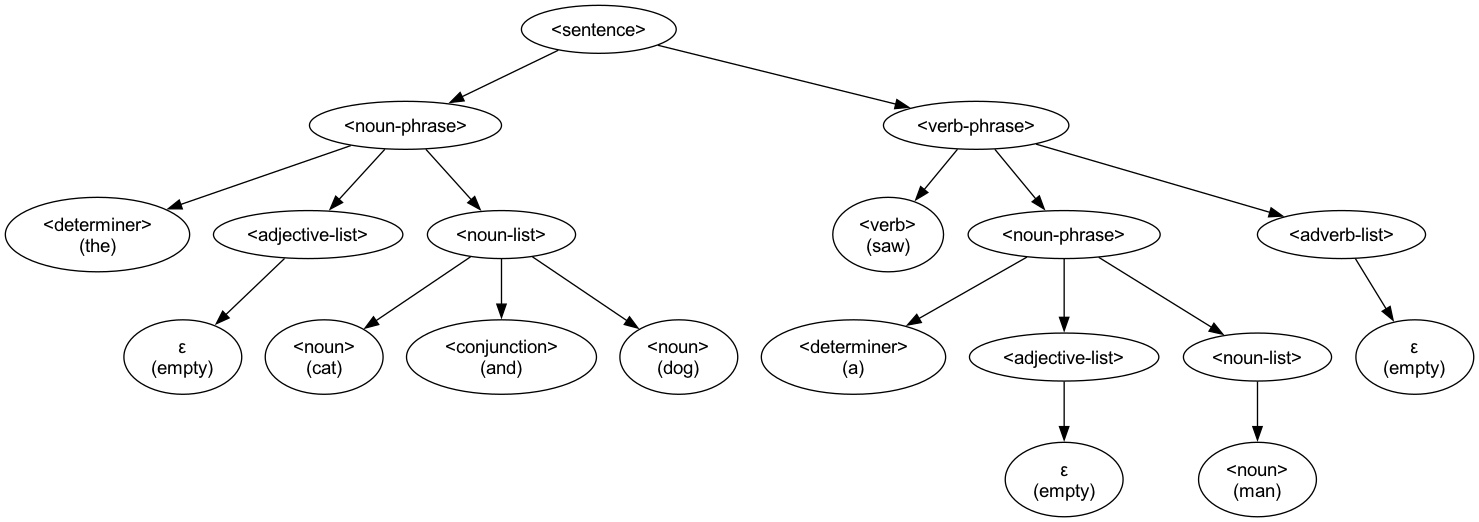
\includegraphics[width=0.85\textwidth]{tree_output_1_sentence_1.png}
    \caption{Sample Parse Tree Visualization}
    \label{fig:sample_tree}
\end{figure}

The findings demonstrate that the Recursive Descent Parser successfully performs syntax analysis, tree generation, and visualization while maintaining modularity and clear error reporting.
	
	\section{Conclusion and Discussion}
	This project successfully demonstrates the implementation of a custom Syntax Analyzer and Parse Tree Visualizer using Python. By utilizing Recursive Descent Parsing techniques, the system effectively validates Context-Free Grammar structures written in BNF notation and generates multiple forms of parse tree representations.

The project combines theoretical concepts from compiler construction and formal language theory with practical software engineering implementation techniques. Support for epsilon productions, graphical AST generation, and detailed error handling mechanisms significantly improve the functionality and usability of the system.

The modular design enables future extensibility and adaptation for more advanced compiler-related applications. Overall, the project provides valuable practical experience in parsing algorithms, recursive programming, data structure management, and syntax analysis systems.
	
	\section*{References}

\begin{enumerate}
    \item Aho, A. V., Lam, M. S., Sethi, R., \& Ullman, J. D. \textit{Compilers: Principles, Techniques, and Tools}. 2nd Edition, Pearson Education, 2006.
    
    \item Hopcroft, J. E., Motwani, R., \& Ullman, J. D. \textit{Introduction to Automata Theory, Languages, and Computation}. 3rd Edition, Pearson, 2006.
    
    \item Python Software Foundation, “Python Documentation.” Available: \url{https://docs.python.org/3/}
    
    \item Graphviz Documentation, “Graph Visualization Software.” Available: \url{https://graphviz.org/}
    
    \item pydot Documentation, “Python Interface to Graphviz.” Available: \url{https://github.com/pydot/pydot}
    
    \item GeeksforGeeks, “Recursive Descent Parser.” Available: \url{https://www.geeksforgeeks.org/recursive-descent-parser/}
\end{enumerate}

	

	
\end{document}